\section{Исследование фонетических закономерностей речевого сигнала}

\subsection{Задание 1.4.1. Гласные фонемы}

Гласные фонемы [а], [о], [у], [э], [ы], [и] записаны в файл
\texttt{sample1.wav} протяжно (по 0,4--0,7 с каждая) с паузами между
звуками. Йотированные буквы «я», «ё», «ю», «е» записаны отдельно в файл
\texttt{sample1b.wav}.

Автоматическая сегментация по энергии (с порогом 8\% от максимального
значения) выделила в \texttt{sample1.wav} шесть фонем, в
\texttt{sample1b.wav} --- четыре. Результаты оценки основной частоты тона
$F_0$ автокорреляционным методом приведены в
таблице~\ref{tab:vowels}; осциллограмма с подписями фонем --- на
рисунке~\ref{fig:vow-wave}.

\begin{table}[H]
	\centering
	\caption{Гласные фонемы: границы и основная частота тона}
	\label{tab:vowels}
	\begin{tabular}{|l|l|l|l|l|}
		\hline
		Фонема & Начало, с & Конец, с & Длительность, с & $F_0$, Гц \\
		\hline
		[а] & 0,70 & 1,37 & 0,67 & 119 \\
		\hline
		[о] & 2,81 & 3,47 & 0,66 & 145 \\
		\hline
		[у] & 4,78 & 5,37 & 0,59 & 172 \\
		\hline
		[э] & 6,99 & 7,57 & 0,58 & 188 \\
		\hline
		[ы] & 8,99 & 9,61 & 0,62 & 205 \\
		\hline
		[и] & 11,22 & 11,66 & 0,44 & 205 \\
		\hline
	\end{tabular}
\end{table}

\begin{figure}[H]
	\centering
	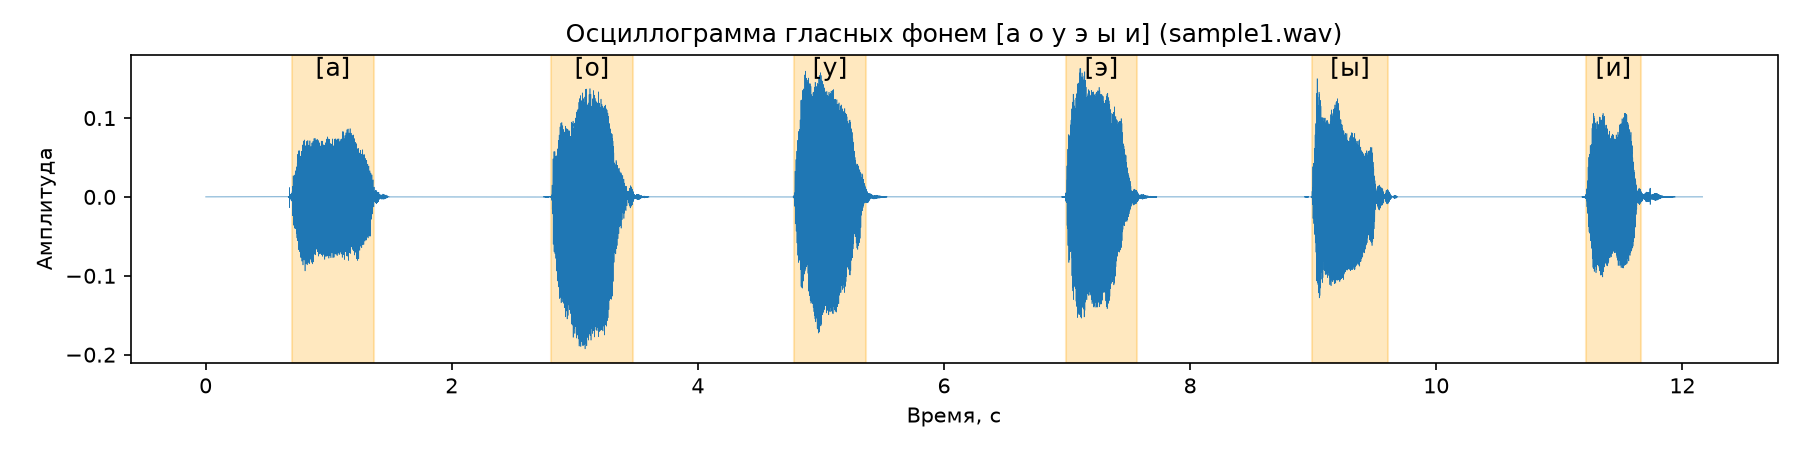
\includegraphics[width=\textwidth]{lab1_sample1_wave.png}
	\caption{Осциллограмма гласных фонем [а о у э ы и]
		(\texttt{sample1.wav})}
	\label{fig:vow-wave}
\end{figure}

На осциллограмме (рис.~\ref{fig:vow-wave}) видно, что каждая гласная
представляет собой квазипериодический фрагмент с плавно изменяющейся
огибающей. Зарисовки огибающих контуров всех шести фонем приведены на
рисунке~\ref{fig:vow-env}: формы огибающих различны и характерны для
каждой фонемы.

\begin{figure}[H]
	\centering
	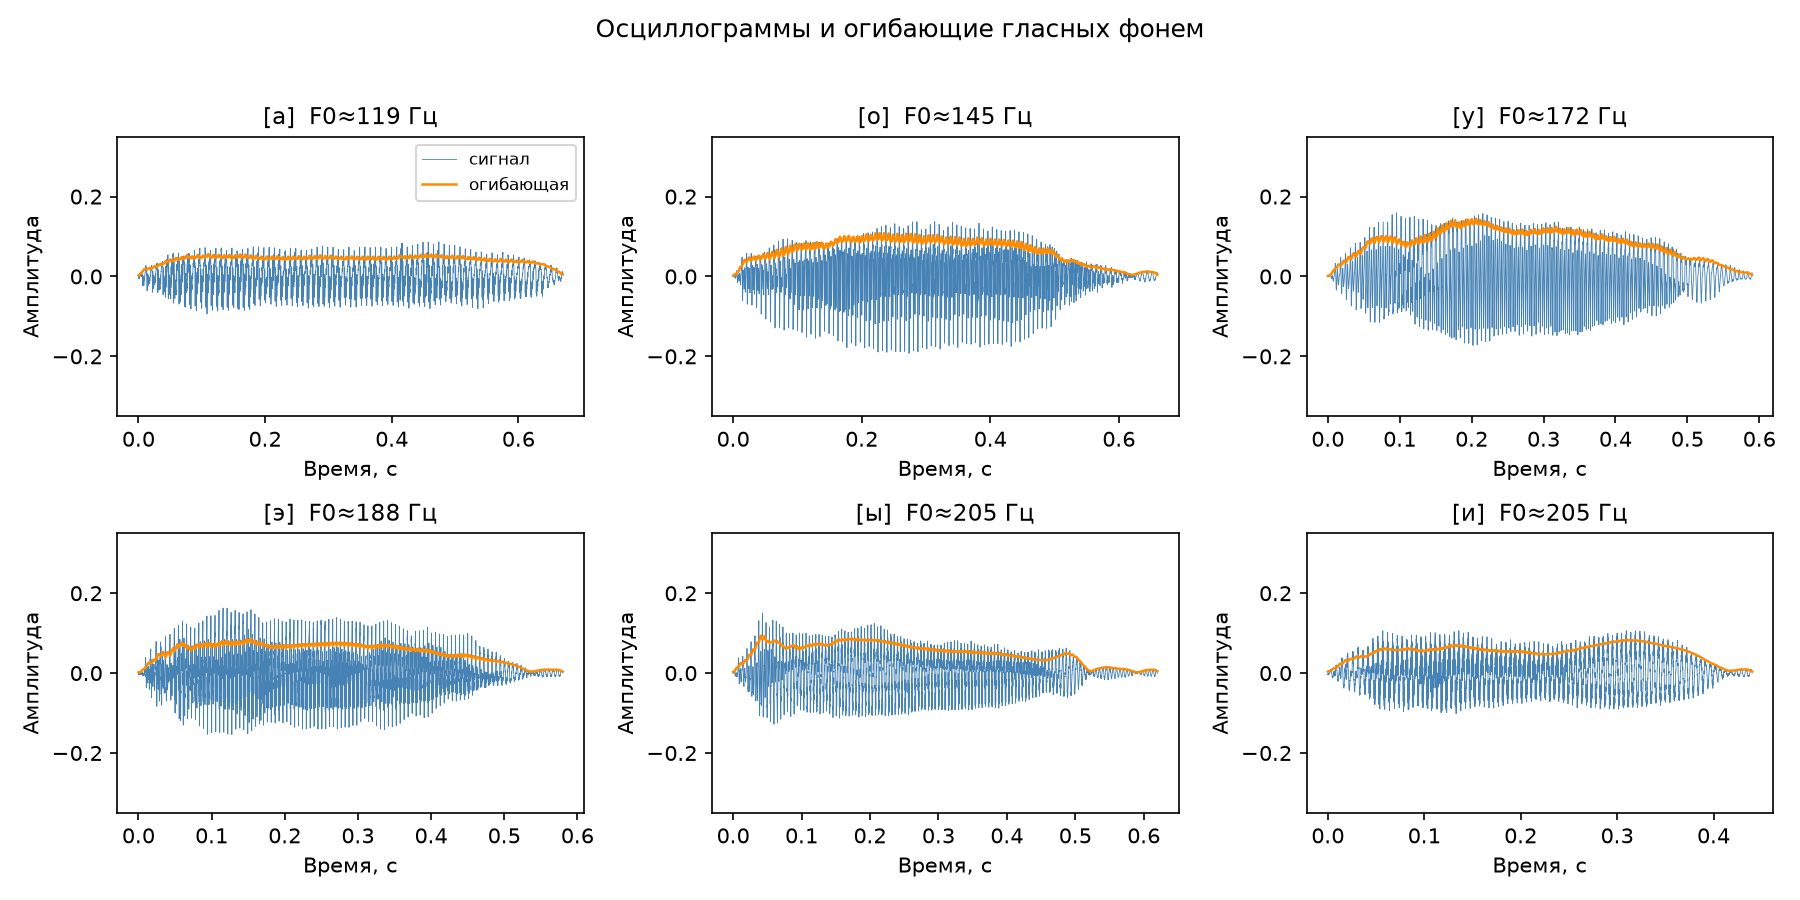
\includegraphics[width=\textwidth]{lab1_vowels_envelopes.png}
	\caption{Осциллограммы и огибающие гласных фонем}
	\label{fig:vow-env}
\end{figure}

Визуальное определение периодичности и последующая оценка
автокорреляционным методом показали, что период фонемы [а] составляет
$T_0 \approx 8{,}4$ мс, что соответствует $F_0 \approx 119$ Гц. На
рисунке~\ref{fig:vow-period} представлены два смежных периода фонемы
[а]; их структура повторяется, что подтверждает квазипериодический
характер сигнала.

\begin{figure}[H]
	\centering
	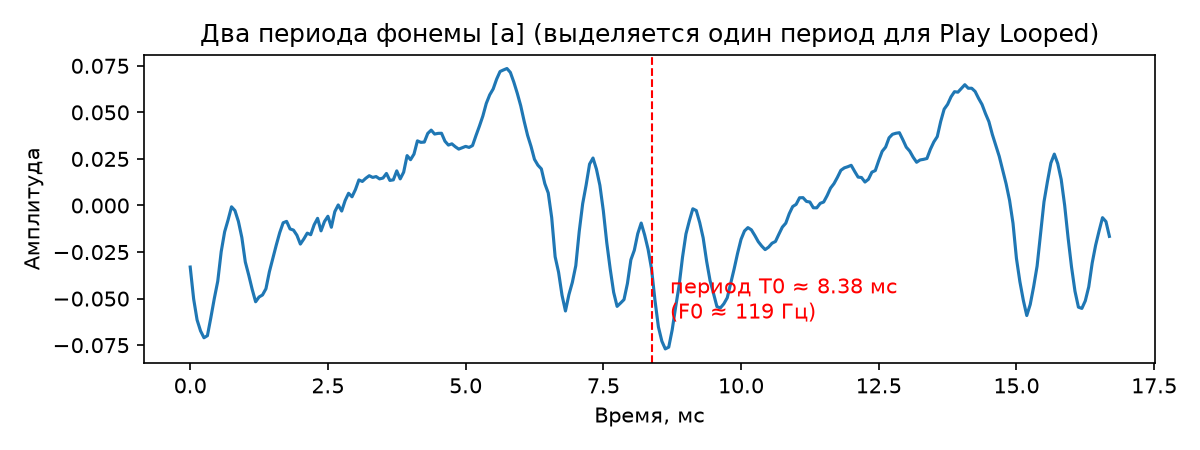
\includegraphics[width=0.8\textwidth]{lab1_vowel_a_period.png}
	\caption{Два периода фонемы [а]; один период выделяется для
		циклического воспроизведения (Play Looped)}
	\label{fig:vow-period}
\end{figure}

Прослушивание выделенного одного периода в одиночном воспроизведении даёт
короткий щелчок (длительность периода всего 8,4 мс). При включении
циклического воспроизведения (Play Looped) слышно подобие произнесённой
гласной [а]: ухо воспринимает периодическую последовательность с
частотой $1/T_0 \approx 119$ Гц, а форма периодика несёт формантные
свойства фонемы.

Спектры всех шести гласных приведены на рисунке~\ref{fig:vow-spec}.
Видна чёткая гармоническая структура: дискретные компоненты на
частотах $F_0$, $2F_0$, $3F_0$\dots с огибающей, образованной формантами
различных фонем.

\begin{figure}[H]
	\centering
	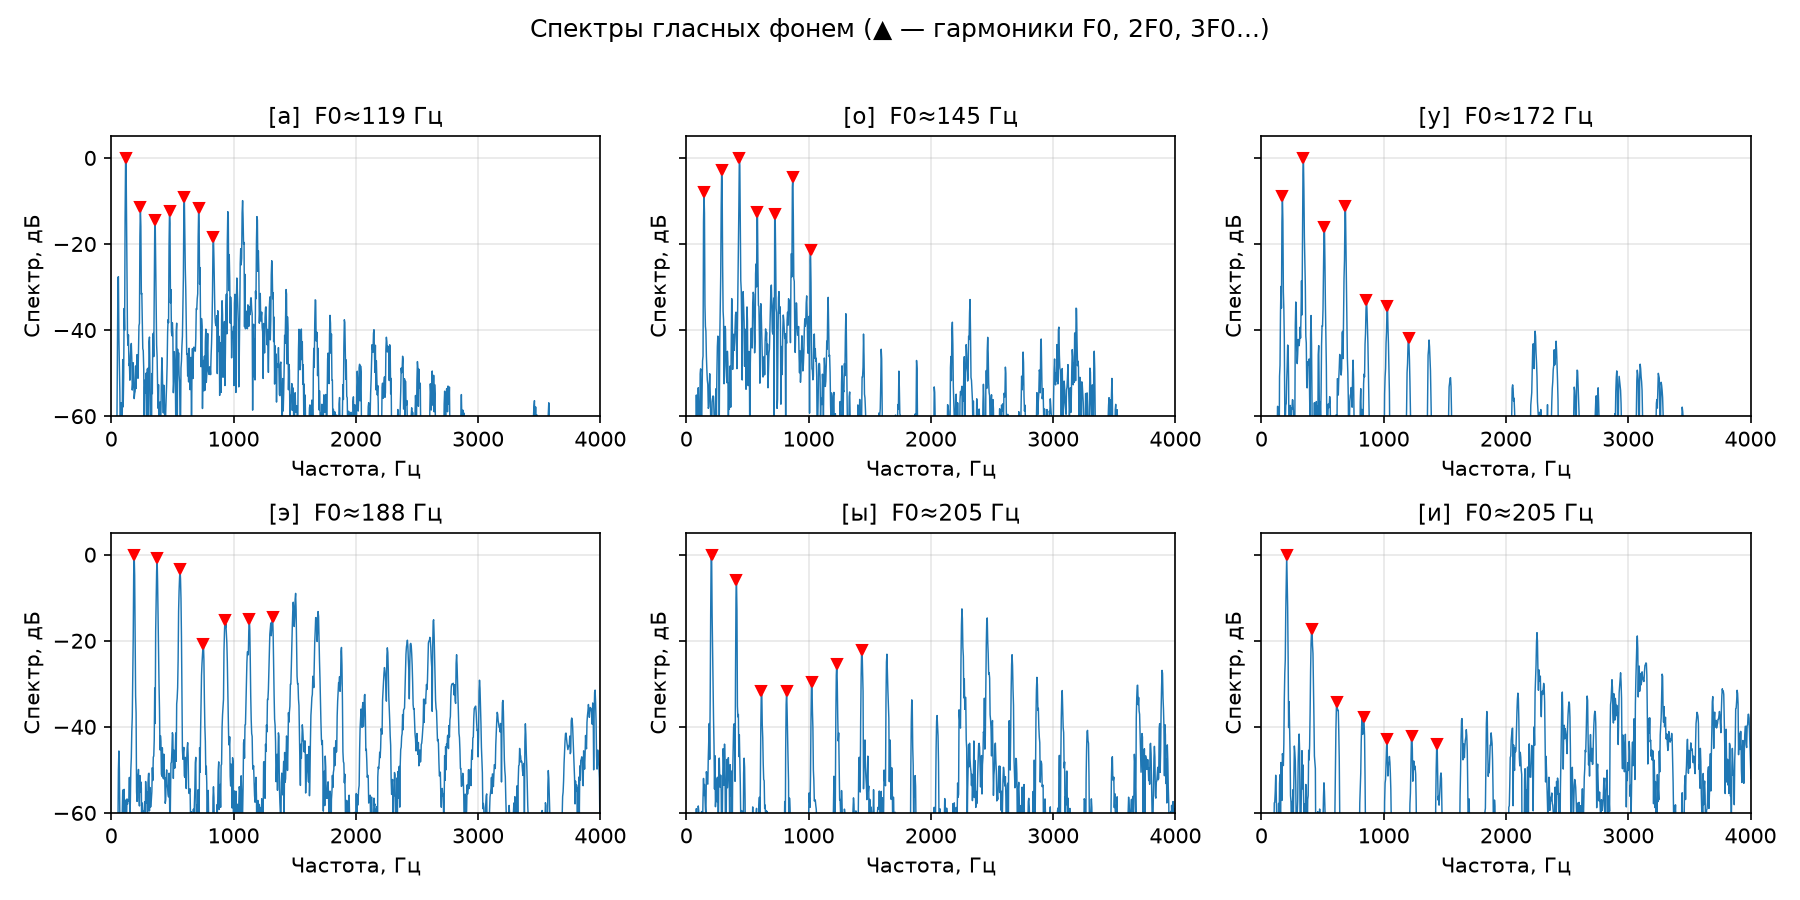
\includegraphics[width=\textwidth]{lab1_vowels_spectra.png}
	\caption{Спектры гласных фонем ($\blacktriangledown$ --- гармоники
		$F_0$, $2F_0$, $3F_0$\dots)}
	\label{fig:vow-spec}
\end{figure}

Йотированные буквы «я», «ё», «ю», «е» записаны в файл
\texttt{sample1b.wav}. Как видно из осциллограмм и спектрограмм
(рис.~\ref{fig:ioted}), каждая из них состоит из двух компонент:
начального скольжения (фонема [й]) и последующей гласной. Спектрограммы
показывают динамику формант на участке скольжения, переходящих в
форманты соответствующей гласной:
\begin{itemize}
	\item «я» $\rightarrow$ [й] + [а];
	\item «ё» $\rightarrow$ [й] + [о];
	\item «ю» $\rightarrow$ [й] + [у];
	\item «е» $\rightarrow$ [й] + [э].
\end{itemize}

\begin{figure}[H]
	\centering
	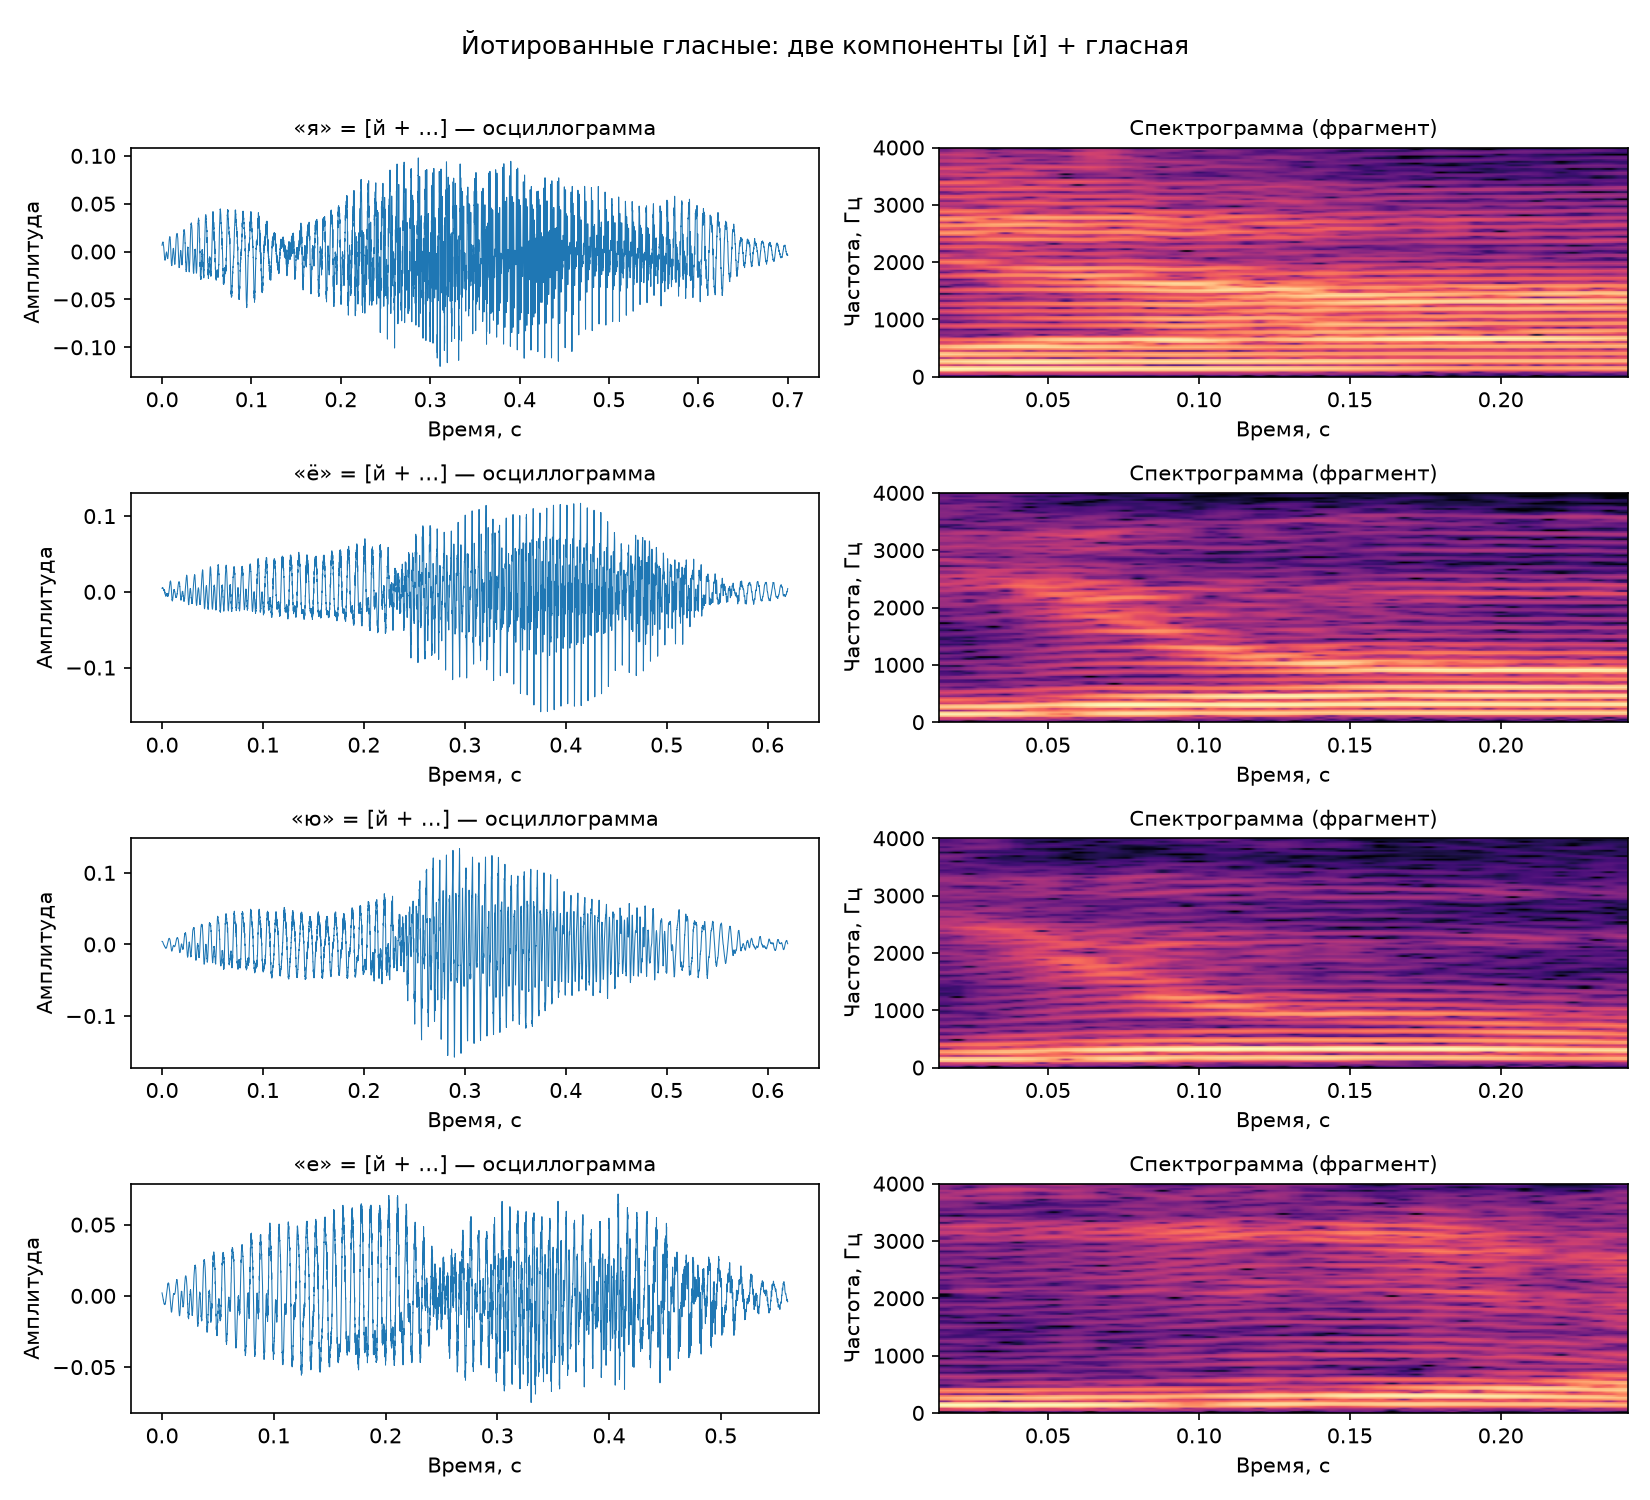
\includegraphics[width=0.95\textwidth]{lab1_ioted.png}
	\caption{Йотированные гласные: две компоненты [й] + гласная}
	\label{fig:ioted}
\end{figure}

\textbf{Выводы по заданию 1.4.1.}
\begin{enumerate}
	\item Гласные фонемы речи разборчиво звучат отдельно от других
		фонем; каждая имеет характерные форму огибающей и набор формант.
	\item Гласные --- квазипериодические сигналы: даже один
		повторяющийся период сигнала в циклическом режиме воспроизведения
		звучит вполне приемлемо (подобие исходной гласной).
	\item Основная частота тона изолированных гласных одной записи
		составила 119--205 Гц.
	\item Буквы «я», «ё», «ю», «е» образуются парами фонем
		[й] + гласная, что подтверждается структурой осциллограмм и
		динамикой формант на спектрограммах.
\end{enumerate}

\subsection{Задание 1.4.2. Шипящие согласные фонемы}

Шипящие согласные [ф], [с], [ш], [х] записаны протяжно в файл
\texttt{sample2.wav}; слоги «фа», «са», «ша», «ха» --- в файл
\texttt{sample3.wav}. Сегментация выделила четыре фонемы в каждом файле.
Осциллограммы приведены на рисунках~\ref{fig:fric-wave}
и~\ref{fig:syll-wave}.

\begin{figure}[H]
	\centering
	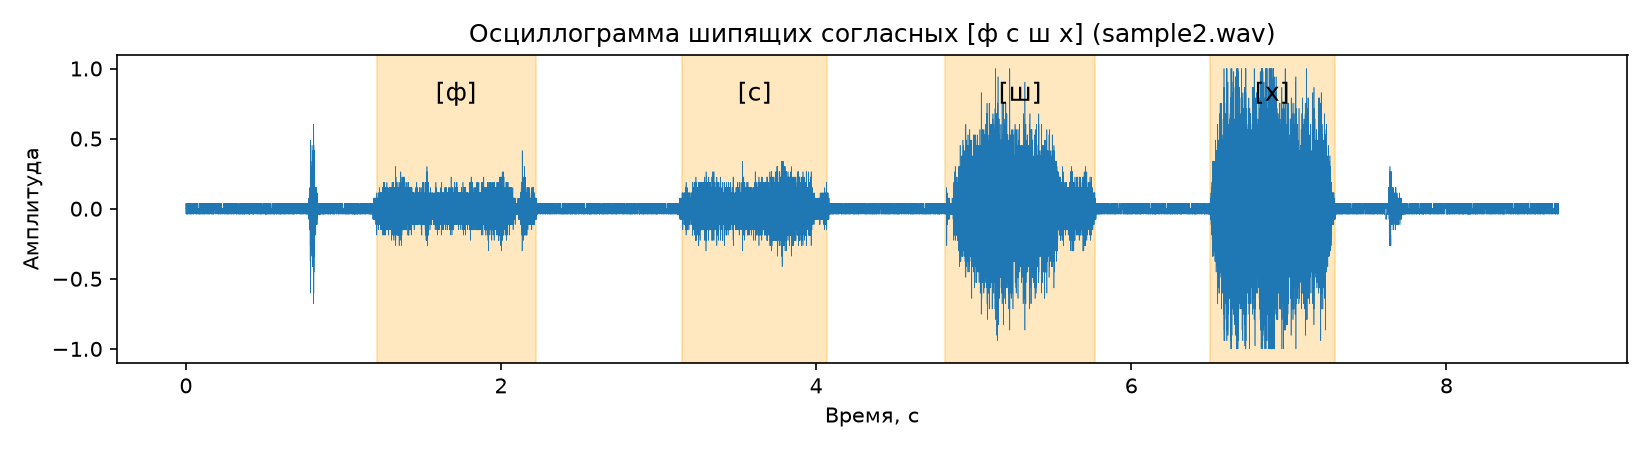
\includegraphics[width=\textwidth]{lab1_fricatives_wave.png}
	\caption{Осциллограмма шипящих согласных [ф с ш х]
		(\texttt{sample2.wav})}
	\label{fig:fric-wave}
\end{figure}

\begin{figure}[H]
	\centering
	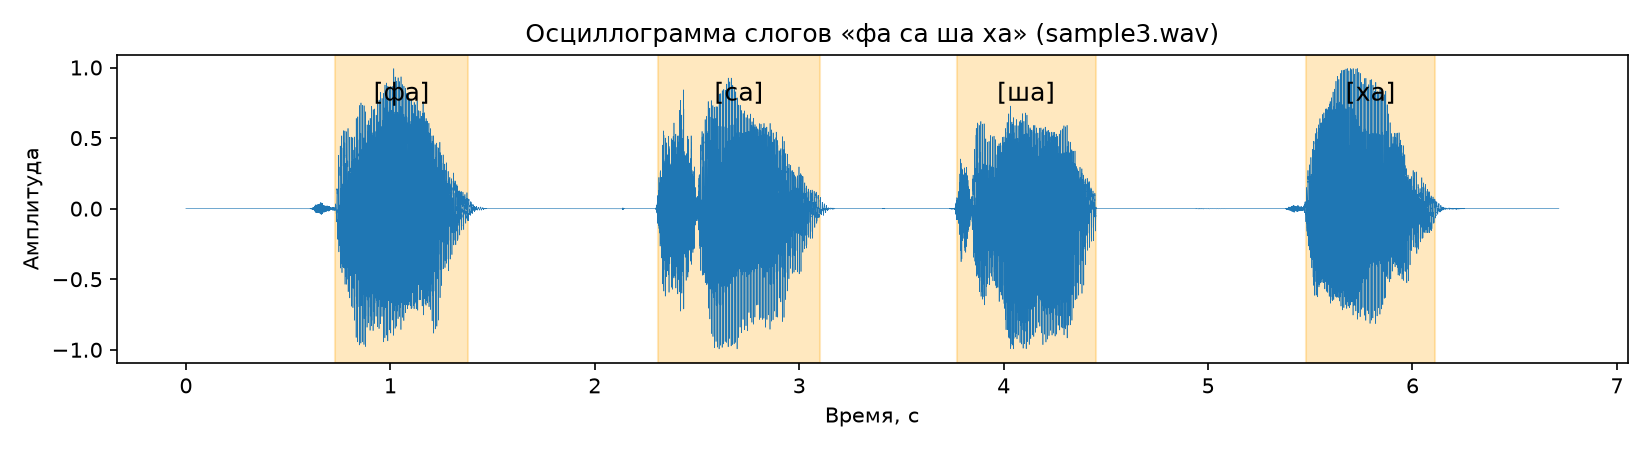
\includegraphics[width=\textwidth]{lab1_syllables_wave.png}
	\caption{Осциллограмма слогов «фа са ша ха» (\texttt{sample3.wav})}
	\label{fig:syll-wave}
\end{figure}

Спектрограммы изолированных шипящих (рис.~\ref{fig:fric-spec})
показывают шумоподобный характер сигнала: горизонтальные полосы
гармоник отсутствуют, энергия распределена по полосе частот,
характерной для каждой фонемы. Спектры (рис.~\ref{fig:fric-spec-sp})
подтверждают различия энергетических профилей: [с] и [ш] концентрируют
энергию в средних и высоких частотах, [х] --- в средней полосе, [ф]
содержит меньше всего энергии.

\begin{figure}[H]
	\centering
	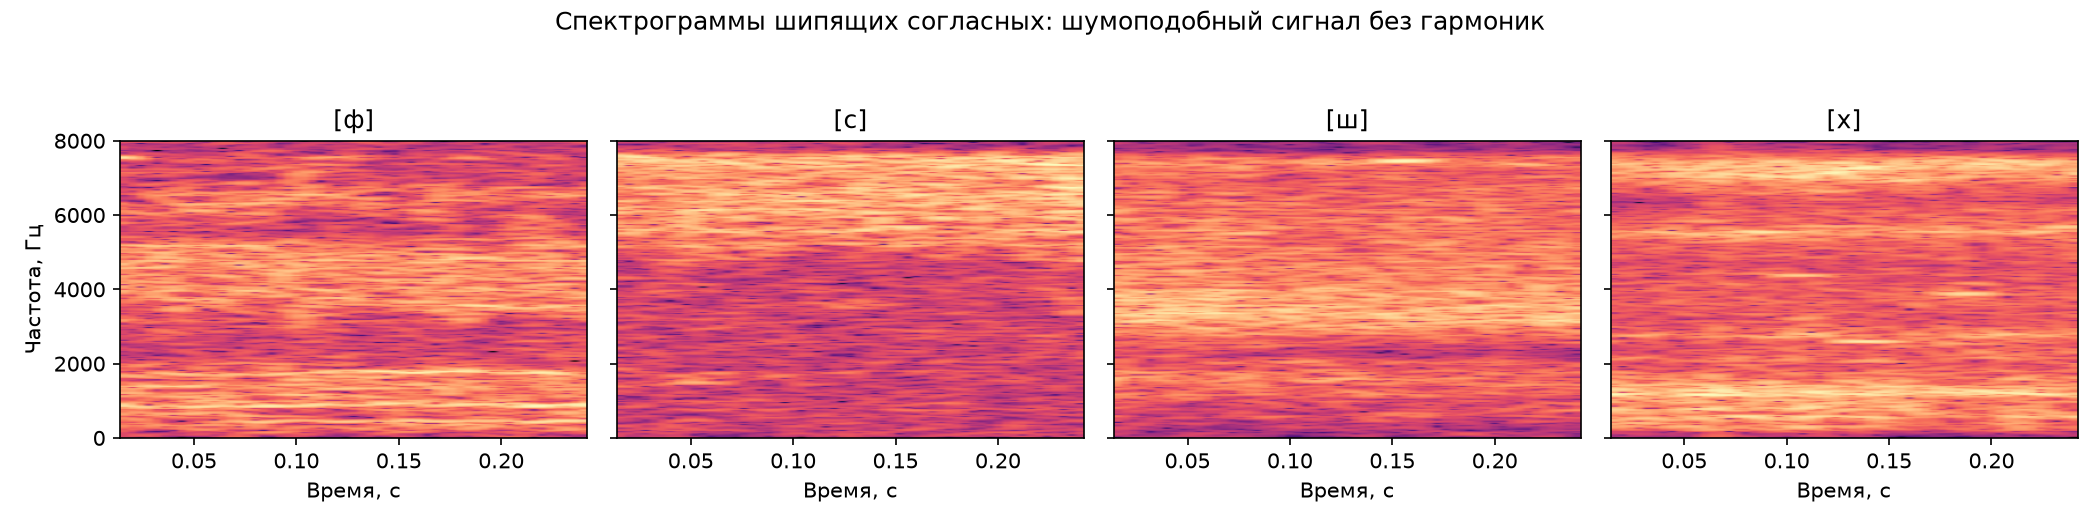
\includegraphics[width=\textwidth]{lab1_fricatives_spectrograms.png}
	\caption{Спектрограммы шипящих согласных: шумоподобный сигнал без
		гармоник}
	\label{fig:fric-spec}
\end{figure}

\begin{figure}[H]
	\centering
	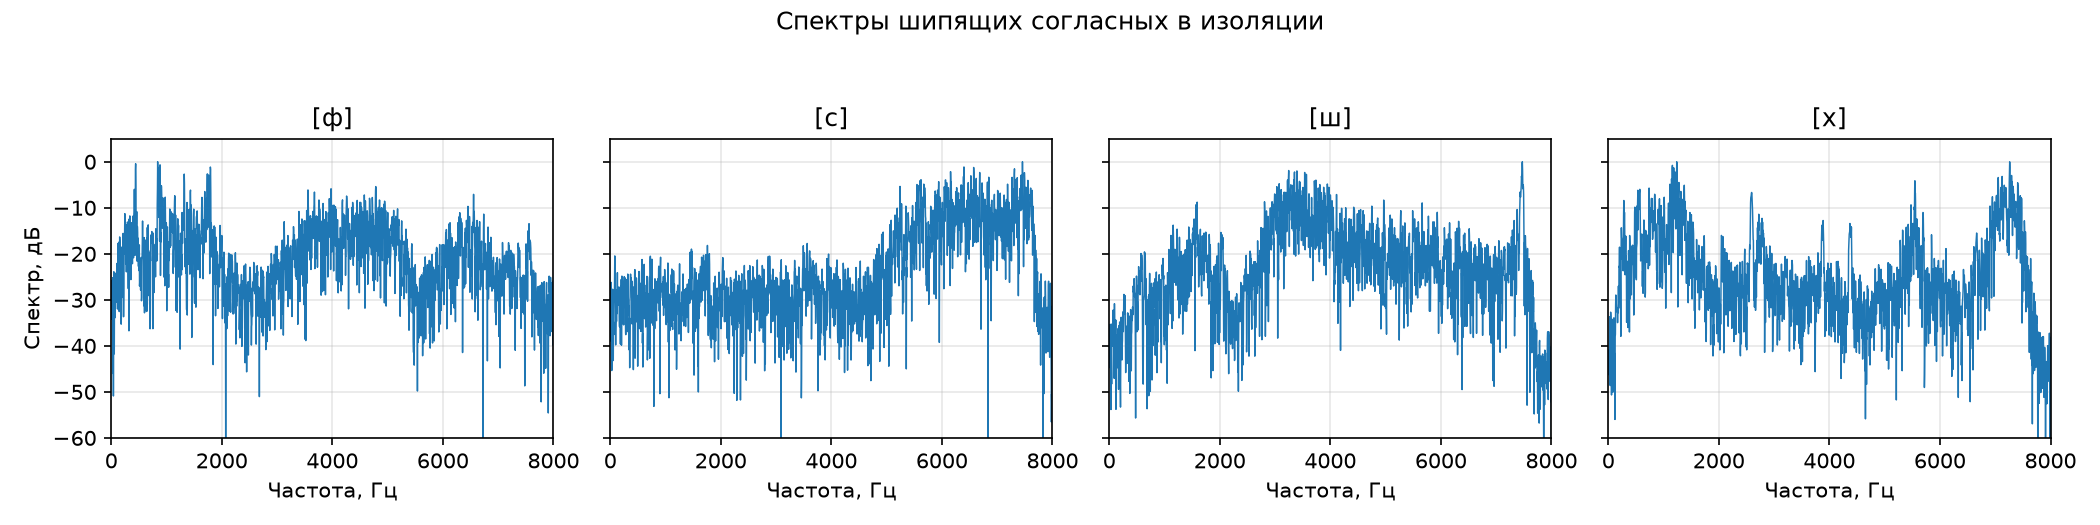
\includegraphics[width=\textwidth]{lab1_fricatives_spectra.png}
	\caption{Спектры шипящих согласных в изоляции}
	\label{fig:fric-spec-sp}
\end{figure}

Количественная оценка периодической составляющей (максимум
нормированной автокорреляционной функции в диапазоне частот 60--400 Гц)
приведена в таблице~\ref{tab:fric}. Значения 0,13--0,30 существенно
меньше типичных значений для гласных (0,8--0,95), что подтверждает
отсутствие выраженной периодичности у шипящих.

\begin{table}[H]
	\centering
	\caption{Шипящие согласные: оценка периодичности сигнала}
	\label{tab:fric}
	\begin{tabular}{|l|l|l|l|}
		\hline
		Фонема & Диапазон, с & Периодичность (АКФ) & Характер \\
		\hline
		[ф] & 1,21--2,22 & 0,30 & шум, периодика слабая \\
		\hline
		[с] & 3,15--4,07 & 0,16 & шум, периодики нет \\
		\hline
		[ш] & 4,82--5,77 & 0,13 & шум, периодики нет \\
		\hline
		[х] & 6,50--7,29 & 0,22 & шум, периодика слабая \\
		\hline
	\end{tabular}
\end{table}

Прослушивание показало, что шипящие согласные можно выделять и
прослушивать отдельно от гласных. В слогах «фа», «са», «ша», «ха»
шипящая у части начала слога, однако её звучание в слоге отличается от
изоляции: накладывается артикуляция соседней гласной
(рис.~\ref{fig:fric-syl}).

\begin{figure}[H]
	\centering
	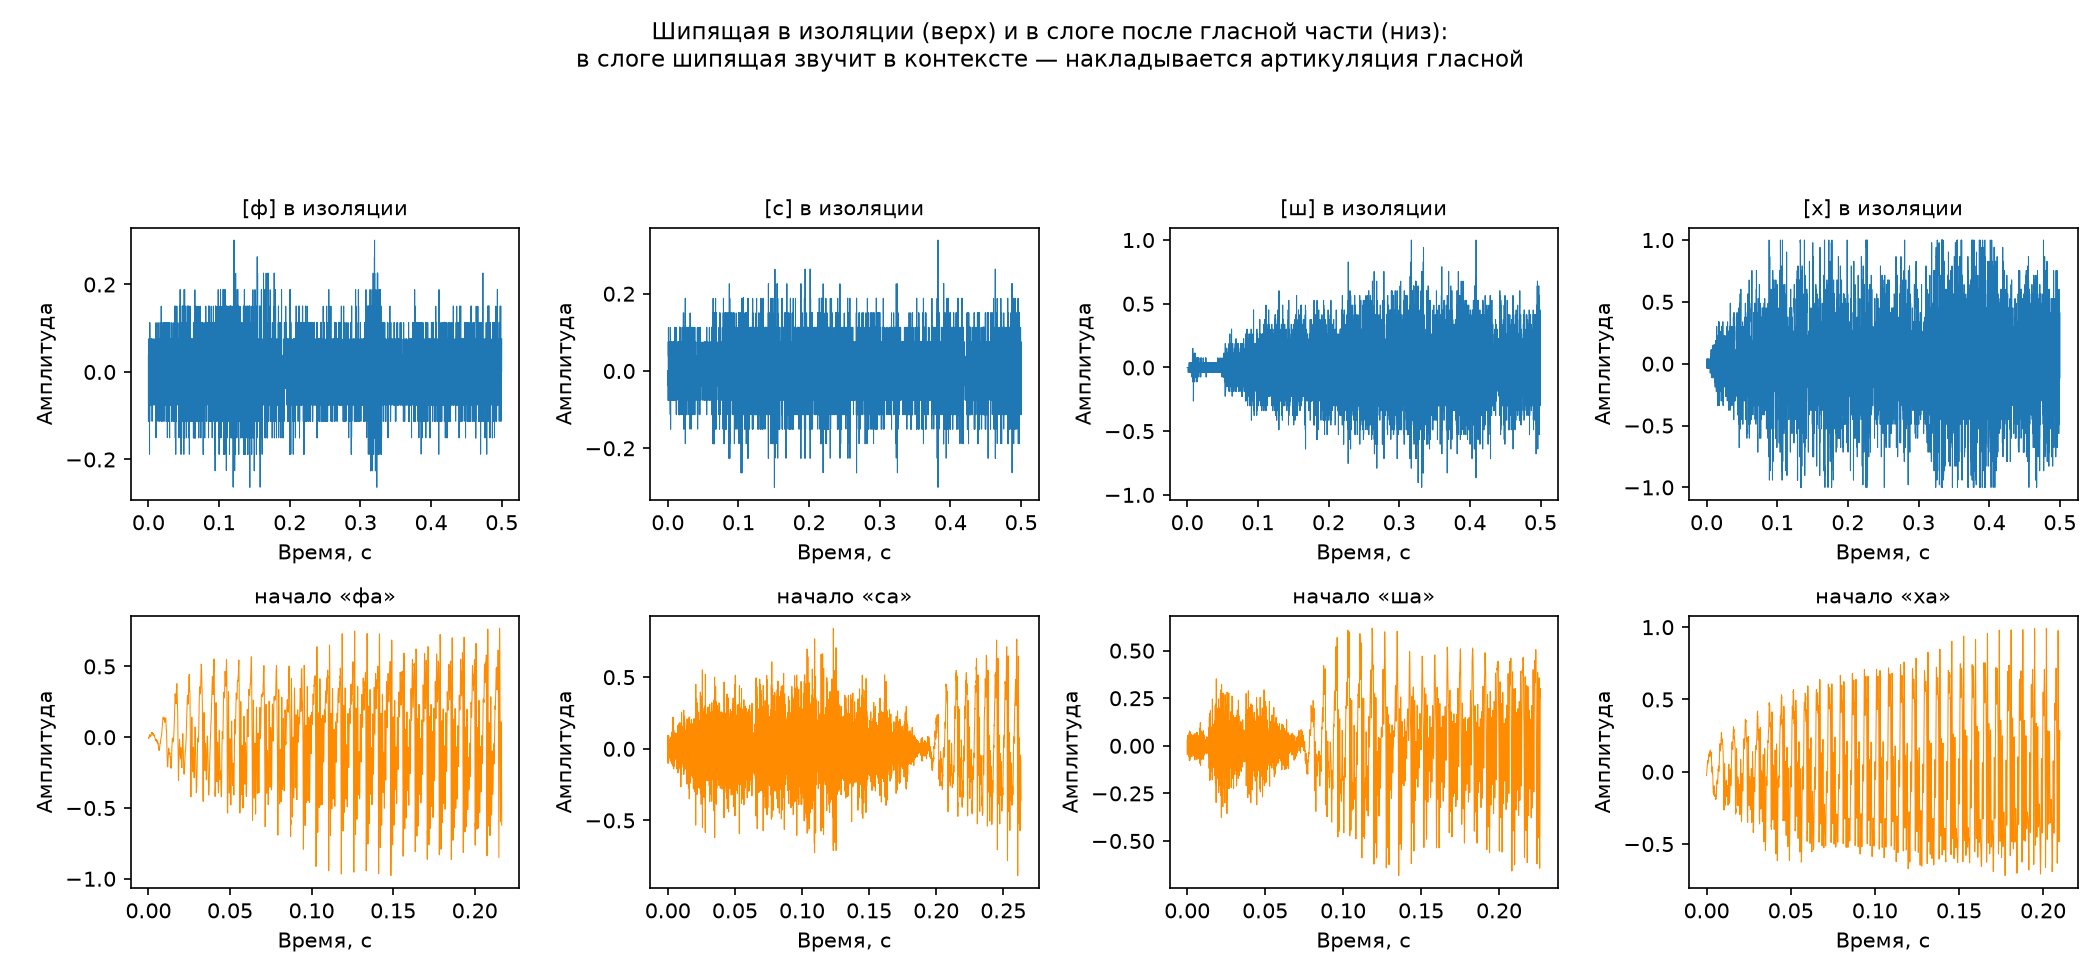
\includegraphics[width=\textwidth]{lab1_fricative_in_syllable.png}
	\caption{Шипящая в изоляции (верхняя строка) и в начале слога
		(нижняя строка): в слоге на шипящую накладывается артикуляция
		гласной}
	\label{fig:fric-syl}
\end{figure}

\begin{figure}[H]
	\centering
	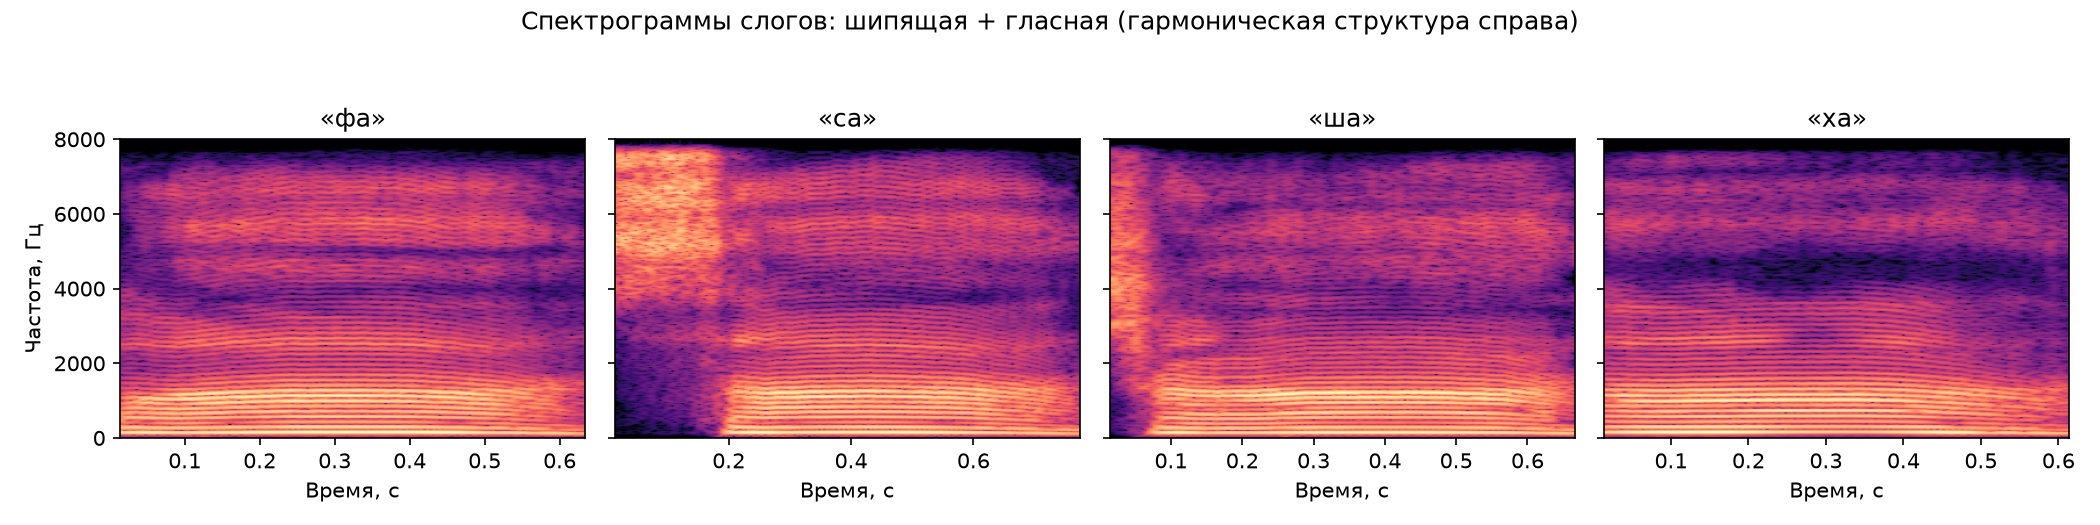
\includegraphics[width=\textwidth]{lab1_syllables_spectrograms.png}
	\caption{Спектрограммы слогов: слева --- шипящая, справа ---
		гармоническая структура гласной}
	\label{fig:syll-spec}
\end{figure}

Попытка выделить отдельный период шипящей согласной и воспроизвести его
циклически (Play Looped) даёт звук, не напоминающий шипящую фонему:
слышен лишь шумовой фрагмент. Это согласуется с результатами
автокорреляционного анализа (таблица~\ref{tab:fric}): периодическая
структура, воспроизводимая зацикливанием, у шипящих отсутствует.

\textbf{Выводы по заданию 1.4.2.}
\begin{enumerate}
	\item Шипящие согласные --- шумоподобные сигналы без выраженной
		гармонической структуры; каждая фонема имеет свой
		энергетический профиль спектра.
	\item Шипящие можно выделять и прослушивать отдельно от гласных,
		однако в слогах их звучание изменяется под влиянием соседней
		гласной (коартикуляция).
	\item Отдельный период шипящей согласной в циклическом режиме
		воспроизведения не звучит как эта фонема --- в отличие от
		гласных, периодическая составляющая у шипящих отсутствует.
\end{enumerate}

\subsection{Задание 1.4.3. Взрывные и носовые согласные}

Взрывные согласные [б], [д] и носовые [м], [н] записаны в файл
\texttt{sample4.wav}, слоги «ба», «да», «ма», «на» --- в файл
\texttt{sample5.wav}. Осциллограммы приведены на
рисунках~\ref{fig:stops-wave} и~\ref{fig:syll2-wave}.

\begin{figure}[H]
	\centering
	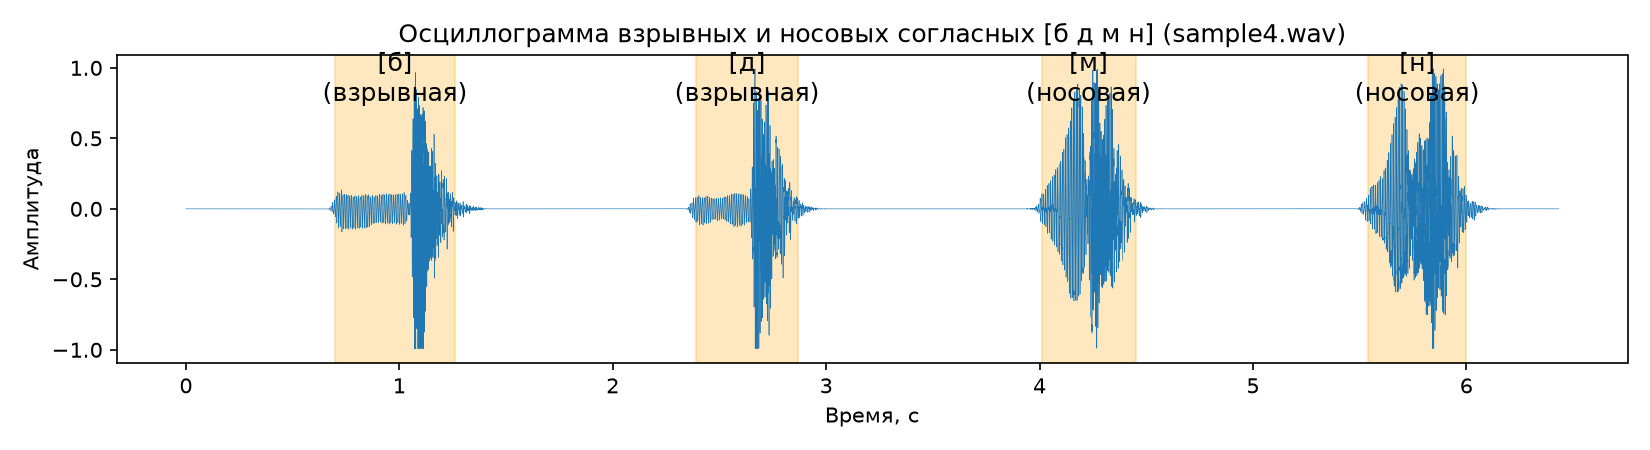
\includegraphics[width=\textwidth]{lab1_stops_wave.png}
	\caption{Осциллограмма взрывных и носовых согласных [б д м н]
		(\texttt{sample4.wav})}
	\label{fig:stops-wave}
\end{figure}

\begin{figure}[H]
	\centering
	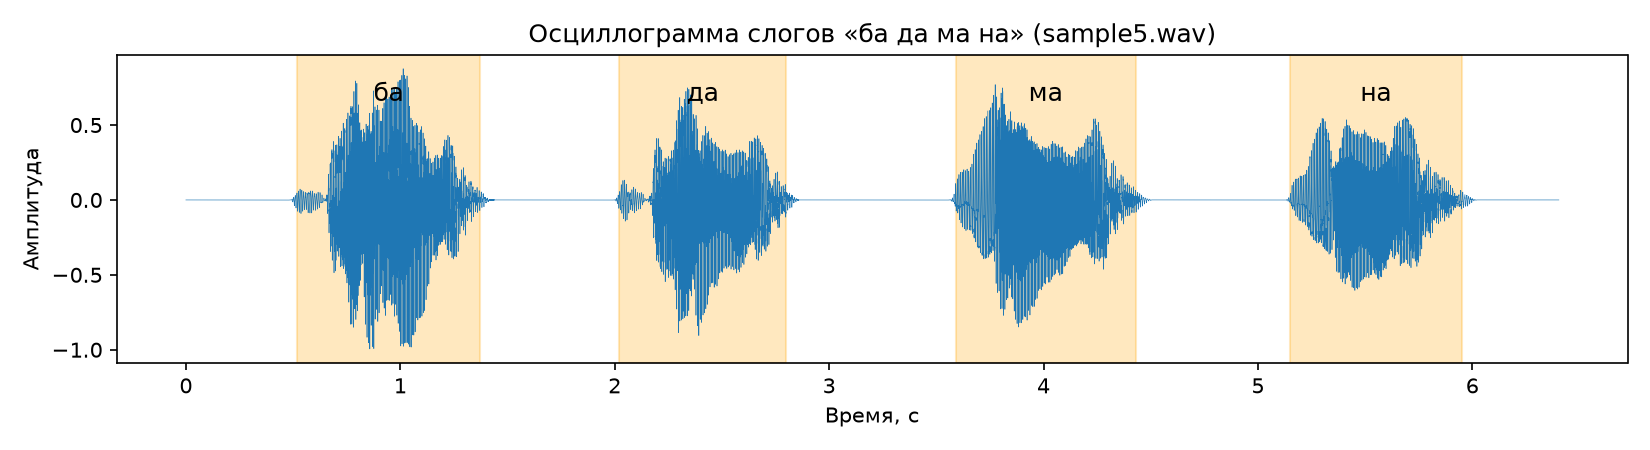
\includegraphics[width=\textwidth]{lab1_syllables2_wave.png}
	\caption{Осциллограмма слогов «ба да ма на» (\texttt{sample5.wav})}
	\label{fig:syll2-wave}
\end{figure}

В изоляции все четыре согласные звучат отдельно
(рис.~\ref{fig:stops-spec}): [б] и [д] --- как короткий взрыв с
последующим голосовым участком, [м] и [н] --- как протяжный носовой
гул. Оценка периодичности (таблица~\ref{tab:stops}) показывает, что
все четыре фонемы содержат выраженную периодическую составляющую
(АКФ 0,61--0,80), поскольку все они звонкие.

\begin{table}[H]
	\centering
	\caption{Взрывные и носовые согласные в изоляции}
	\label{tab:stops}
	\begin{tabular}{|l|l|l|l|l|l|}
		\hline
		Фонема & Тип & Диапазон, с & Длит., с & Периодичность & $F_0$, Гц \\
		\hline
		[б] & взрывная & 0,70--1,26 & 0,56 & 0,80 & 121 \\
		\hline
		[д] & взрывная & 2,39--2,87 & 0,48 & 0,64 & 123 \\
		\hline
		[м] & носовая & 4,01--4,45 & 0,44 & 0,61 & 163 \\
		\hline
		[н] & носовая & 5,54--6,00 & 0,46 & 0,80 & 158 \\
		\hline
	\end{tabular}
\end{table}

\begin{figure}[H]
	\centering
	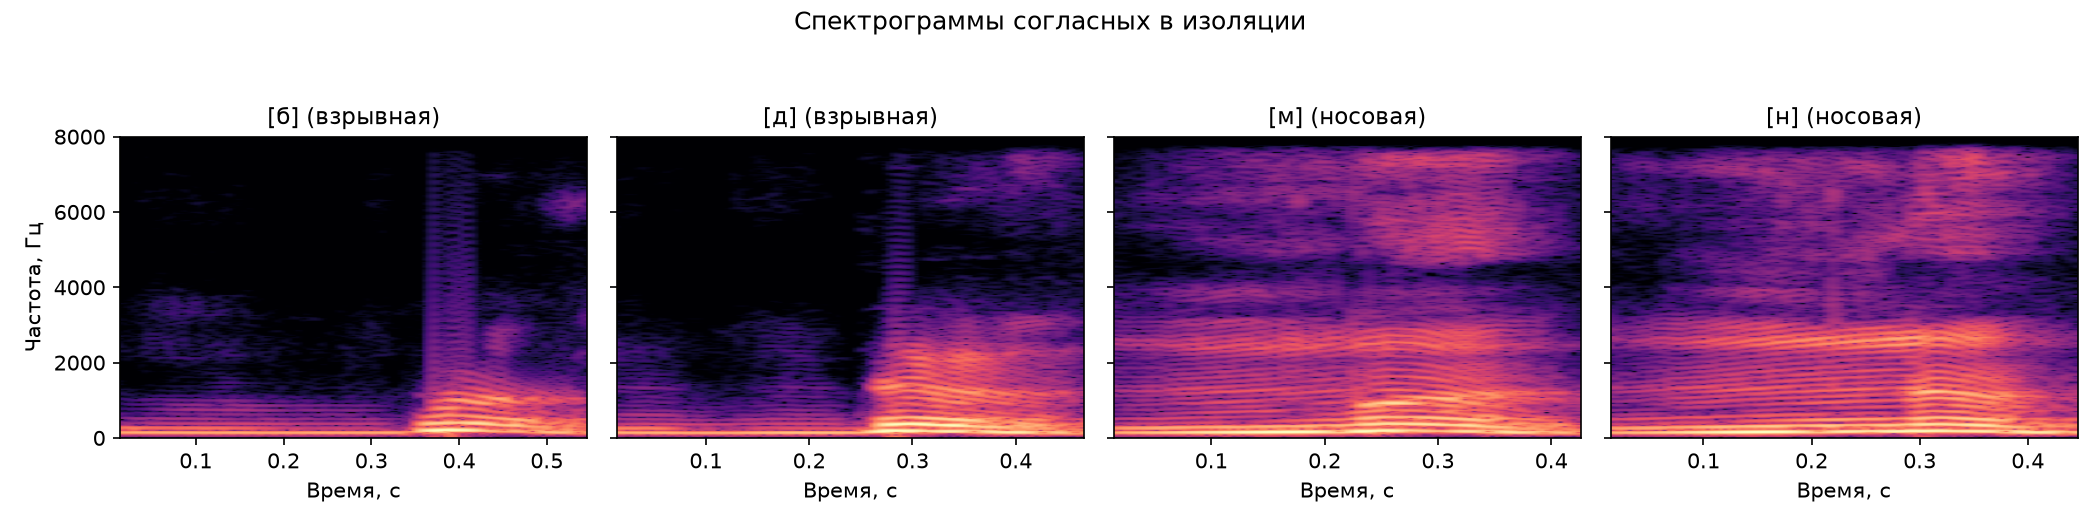
\includegraphics[width=\textwidth]{lab1_stops_spectrograms.png}
	\caption{Спектрограммы взрывных и носовых согласных в изоляции}
	\label{fig:stops-spec}
\end{figure}

В слогах «ба», «да», «ма», «на» картина меняется
(рис.~\ref{fig:syll2-spec}). Спектрограммы показывают:
\begin{itemize}
	\item в «ба» и «да» перед формантами гласной [а] расположен
		короткий участок взрывной согласной, граница которого
		прослеживается слабо;
	\item в «ма» и «на» носовой гул плавно переходит в гласную без
		чёткой границы.
\end{itemize}

\begin{figure}[H]
	\centering
	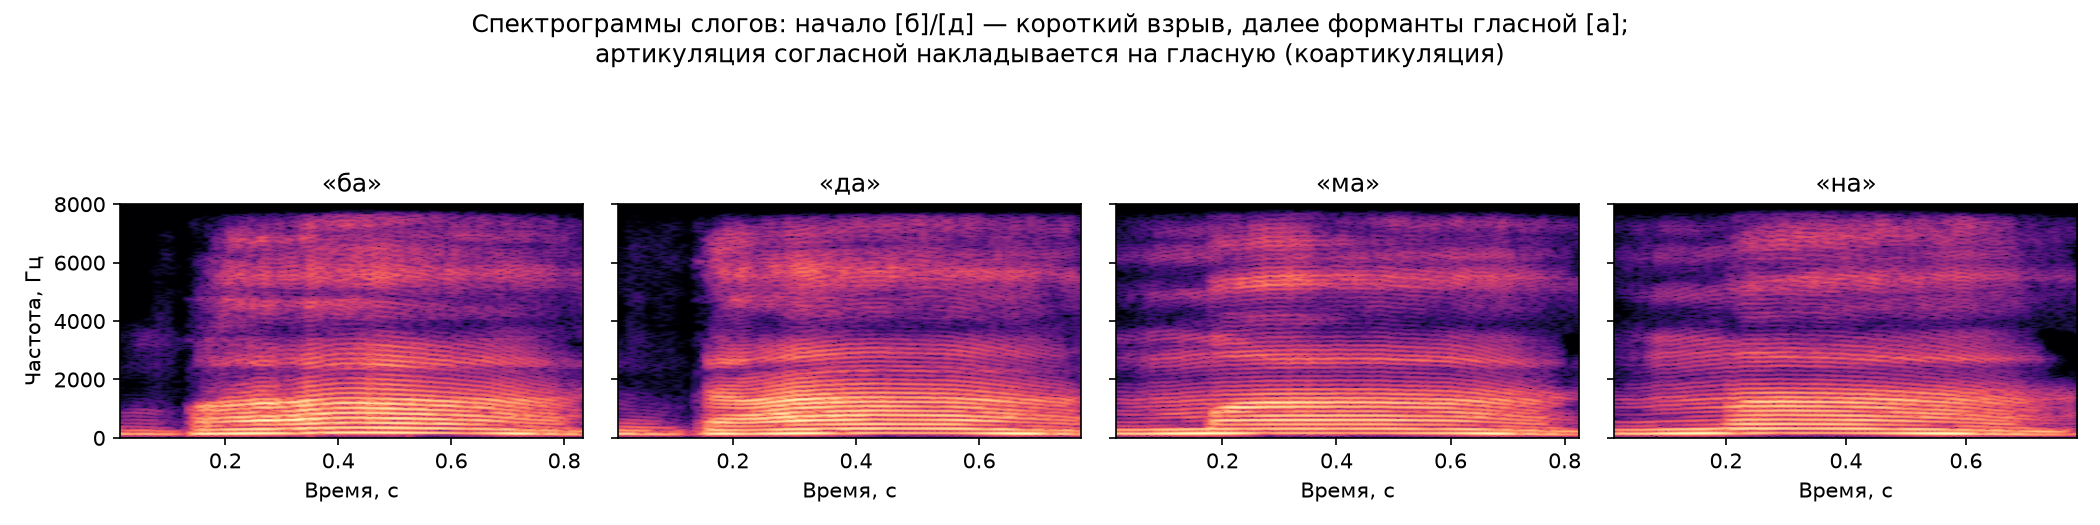
\includegraphics[width=\textwidth]{lab1_syllables2_spectrograms.png}
	\caption{Спектрограммы слогов «ба да ма на»: артикуляция согласной
		накладывается на гласную (коартикуляция)}
	\label{fig:syll2-spec}
\end{figure}

Детальный вид начала слогов «ба» и «да» (рис.~\ref{fig:coart})
показывает, что попытка вырезать участок, соответствующий взрывной
согласной, не позволяет услышать изолированный [б] или [д]: их
артикуляция «влилась» в соседний гласный звук [а]. То же относится к
носовым согласным в слогах «ма» и «на».

\begin{figure}[H]
	\centering
	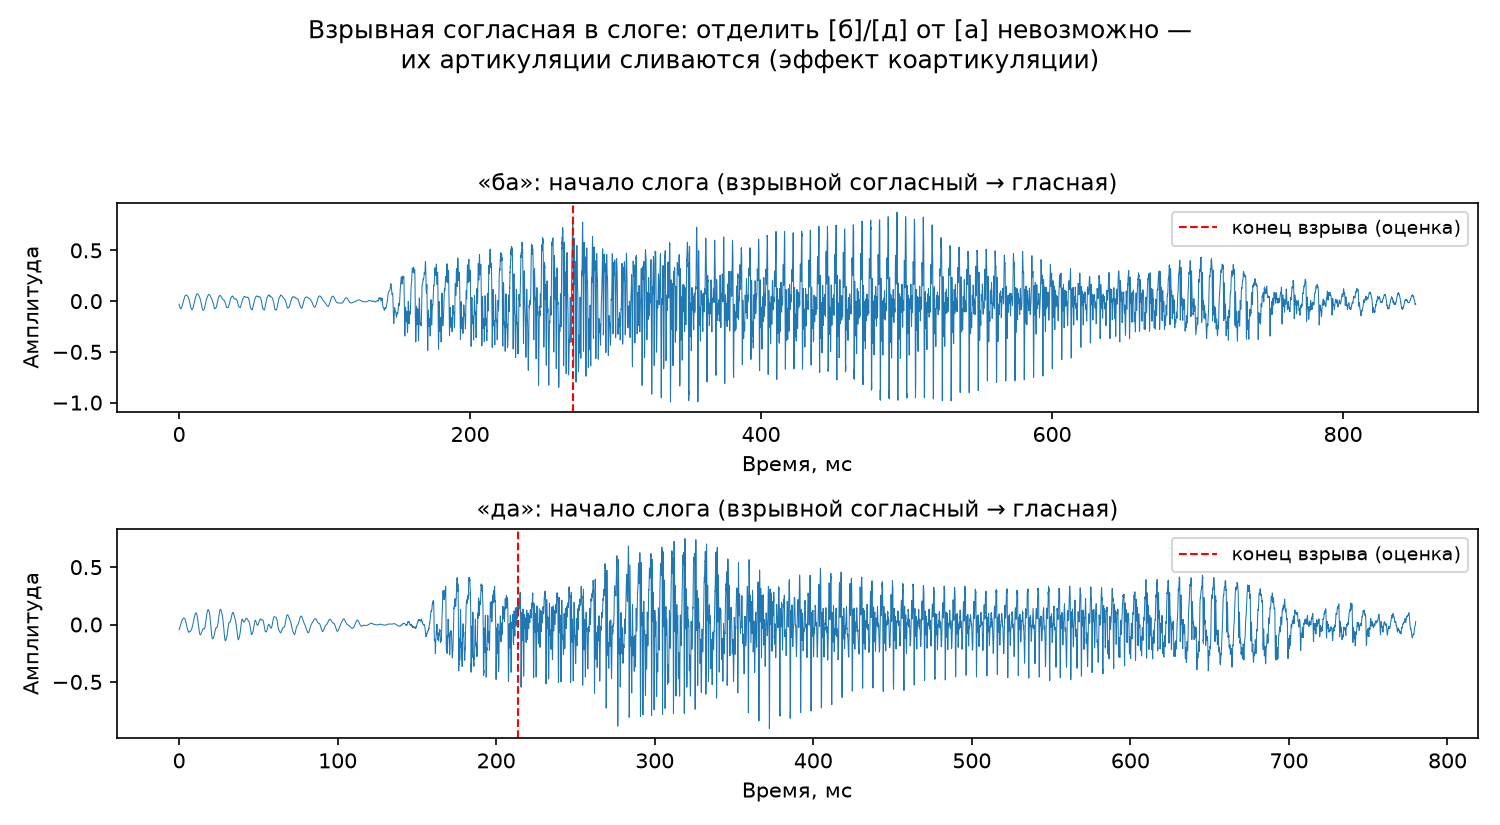
\includegraphics[width=0.95\textwidth]{lab1_coarticulation.png}
	\caption{Начало слогов «ба» и «да»: отделить [б]/[д] от [а]
		невозможно --- артикуляции сливаются (эффект коартикуляции)}
	\label{fig:coart}
\end{figure}

\textbf{Выводы по заданию 1.4.3.}
\begin{enumerate}
	\item В изоляции взрывные [б], [д] и носовые [м], [н] звучат
		отдельно и содержат периодическую составляющую (все они
		звонкие).
	\item В слогах «ба», «да», «ма», «на» выделить и прослушать
		согласную отдельно от гласной не удаётся: происходит наложение
		артикуляции одного звука на другой --- эффект коартикуляции.
	\item Таким образом, все согласные звуки звучат в контексте
		с гласными; отдельно периодически звучащие гласные и
		периодическая составляющая звонких согласных существенно
		отличаются по звучанию от согласных в слогах.
\end{enumerate}
